

In this section we demonstrate that the proof system presented in section \ref{sect:proofSystem} is sound. 
For this, we give a stronger, deeper meaning to our Hoare tuples  (Sect \ref{s:deep:valid}), which requires that \se{satisfaction} of assertions is preserved from the perspective of several frames, rather than just the top frame.

% In Sect.  \ref{s:deep:mean} we define deep satisfaction of assertions. 
% In Sect \ref{sect:HLmeans} we define deep satisfaction of specifications.
% We give the usual meaning to the Hoare triples (Sect \ref{sect:HLmeans}), in a deep as well as shallow version,
We prove soundness of of Hoare triples (Sect \ref{sect:prove:triples:sound}).
We then show how execution starting from some external state can be summarised into purely external execution and terminating execution of public methods (Sect \ref{sect:termExecs}). We then use these decompositions and a well-founded ordering to prove soundness of our quadruples  and of the overall system (Sect \ref{sect:prove:sound:quadruples}).


\subsection{Deep Satisfaction} 
\label{s:deep:valid}
% SOME MOVED

As we saw in section \ref{s:viewAndProtect}, it is possible  for an assertion to hold in some state,  but no longer hold after popping the top frame from the stack. 
This has implications for the appropriate meaning of Hoare tuples:

\begin{example}
\label{ex:motivate:deep}
Assume state $\sigma_a$, such that $\interpret {\sigma_a} {\prg{this}}=o_1$, $\interpret {\sigma} {\prg{this}.f}=o_2$, $\interpret {\sigma} {x}=o_3$, $\interpret {\sigma} {x.f}=o_2$,  
and $\interpret {\sigma} {x.g}=o_4$, where $o_2$ is external and all other objects are internal. 
We then have $..,\sigma_a \models  \inside {o_4}$.
Assume that the continuation of $\sigma_a$   consists of a method $x.m()$. Then,
upon entry to that method, when we push the new frame, we have a state $\sigma_b$, which also satisfies $..,\sigma_a \models  \inside {o_4}$.
Assume that the   body of $m$ is $\prg{this}.f.m1(\prg{this}.g); \prg{this}.f := \prg{this};  \prg{this}.g := \prg{this}$, and that the external method $m1$ stores in the 
receiver a reference to the argument.
Then, at the end of method execution, and before popping the stack, we have a state $\sigma_c$, which also satisfies $..,\sigma_c \models  \inside {o_4}$.
However, after we pop the stack, we obtain $\sigma_d$, for which $..,\sigma_d \not\models  \inside {o_4}$.
\end{example}
 

To address this problem, we introduce ``deep satisfaction'' of assertions $ \satDAssertFrom M  \sigma k   A$ which says that $A$ is satisfied in $\sigma$  in all frames of $\sigma$ from $k$ onwards, 
\ie  $ \satDAssertFrom M  \sigma k   A$ iff $\sigma = ((\phi_1\cdot ... \phi_n), \chi)$ and $k\leq n$ and $\forall j. [\  k\leq j \leq n \ \Rightarrow \ M, ((\phi_1\cdot ... \phi_j), \chi) \models A'\ ]$ where $A'$ is $A$ where all free variables have been substituted according to $\phi_n$ -- \cf Def. \ref{def:restrict}.
We then introduce ``deep'' quadruples,   $\satisfiesD {M} {\quadruple  {A} }   {\sigma}   {A'} {A''}$ , which promise that if $\sigma$ satisfies $A$ from $k$ onwards, then, and executes its continuation to termination, then the final state will satisfy $A'$ from $k$ onwards, and also, all intermediate external states will satisfy $A''$ from $k$ onwards - \cf Def \ref{def:restrict}.
We define   $\satisfiesD {M} {\quadruple  {A} }   {stmt}   {A'} {A''} $ and  $\satisfiesD {M} {S}$ accordingly.


Thus. continuing with example \ref{ex:motivate:deep},  we have that\ \  $\satisfies {M} {\quadruple   {\inside {o_4}} }   {\sigma_b}   {\inside {o_4}}  {true} $, \ \ 
 but \\ $\notSatisfiesD {M}   {\quadruple   {\inside {o_4}} }  {\sigma_b}   {\inside {o_4}}  {true}  $.
\ \  In general, deep satisfaction is stronger than shallow:   
 
\begin{lemma}[Deep   vs Shallow Satisfaction]
For all $M$, $A$, $A'$, $A''$, $\sigma$, $stmt$, and $S$
\begin{itemize}
\item
 $\satisfiesD {M} {\quadruple  {A} }   {\sigma}   {A'} {A''}   \ \ \ \Longrightarrow \ \ \   \satisfies {M} {\quadruple  {A} }   {\sigma}   {A'} {A''}$

\item
 $\satisfiesD {M} {\quadruple  {A} }   {stmt}   {A'} {A''}   \ \ \ \Longrightarrow \ \ \   \satisfies {M} {\quadruple  {A} }   {stmt}   {A'} {A''}$
\item 
$\satisfiesD {M} {S}  \ \ \ \Longrightarrow \ \ \ \satisfies {M} {S}$
\end{itemize}
\end{lemma}


%%%%%%%%%%%%%%%%%%%%%%%%%%%%%%%%%%%%%%%%%%%%%%%%%%%

 
%%%%%%%%%%%%%%%%%%%%%%%%%%%%%%%%%%%%%%%%%%%%%%%%%%%

\subsection{Soundness of the Hoare Triples Logic}

We require  that the supporting proof system for assertions, $M\vdash A$, and the  underlying Hoare logic, $M\ \vdash_{ul}\  \triple A {stmt} {A'}$, are sound:
\begin{axiom}
\label{lemma:axiom:enc:assert:ul}
\label{ax:ul:sound}
We require for all $M$, $A$, $A'$, $stmt$:
\begin{center}
$M \vdash A   \ \ \ \  \Longrightarrow  \ \ \ \  \forall \sigma.[\ M, \sigma \models A\ ]$.\\
% \end{center}
%\end{axiom}
%
%\noindent
%Moreover, we assume that the  \ie for all $A$, $A'$, $stmt$:\ \ \  
%
%\begin{axiom}
% \begin{center}
{$M\ \vdash_{ul}\  \triple A {stmt} {A'}  \ \ \ \  \Longrightarrow  \ \ \ \ \satisfies  {M} { \triple A {stmt} {A'}}$ }
 \end{center}
\end{axiom}

\noindent
\label{sect:prove:triples:sound}
We prove various properties about protection
\cf section \ref{s:app:protect:lemmas}.
Using these lemmas. we prove soundness of the inference system for triples $M \vdash  \triple A {stmt} {A'} $ -- \cf \A, \ref{s:sound:app:triples}.

 
 


\begin{Theorem}
\label{l:triples:sound}
For module  $M$ % and $\Mtwo$, 
such that  $\vdash M$, and for any assertions $A$,  $A'$, $A''$ and statement  $stmt$:
\begin{center}
$M\ \vdash\  \triple A {stmt} {A'}  \ \ \ \  \Longrightarrow  \ \ \ \ \satisfiesD {M} {\quadruple {A} {stmt} {A'} {A''}}$
\end{center}
\end{Theorem}
 



\subsection{Soundness of the Hoare Quadruples, and of the overall System}

For the soundness proof of our quadruples we need to address two challenges. 
First, that we need to apply induction on the execution, as well as on the Hoare logic proof. 
Second, that execution of an external call may consist os any number of external steps, interleaved with calls of public, internal methods, which in their turn may may make external calls, leading to further calls of public methods.


We address the first challenge  through the definition of a well-founded ordering (\cf Section \ref{sect:prove:wellfounded}). 
We address the second challenge by introducing summarized executions, which essentially collapse all oublic, internal method calls into one large step (\cf Section \ref{sect:termExecs}).

\subsubsection{A well-founded ordering}
\label{sect:prove:wellfounded}

We define that $(A_1,\sigma_1,A_2, A_3) \ll_{M,\Mtwo}  (A_4,\sigma_2,A_5, A_6)$ if $\sigma_1$ executes to terminations in fewer steps than $\sigma_2$ (we consider   scoped exercution,
\ie execution of the continuation of the top frames, and consider the shortest terminating execution), or  the proof of $M \vdash \quadruple {A_1} {\sigma.\prg{cont}} {A_2} {A_3} $
is shallower than the the proof of  $M \vdash \quadruple {A_4} {\sigma.\prg{cont}} {A_5} {A_5} $ (we consider the shallowest possible proofs). Full Def. in \ref{def:measure}.

 

 


\begin{auxLemma}
\label{lemma:normal:two}
For any modules $M$ and $\Mtwo$,  the relation $\_ \ll_{M,\Mtwo}  \_$ is well-founded.
\end{auxLemma}

%%%%%%%%%%%%%%%%%%%%%%% S U M M A R I E S of exectuon %%%%%%%%%%%%%%%%%%%%%%%%%%%%%%%%%%%%%%%%%%%%% 
\subsubsection{Summarised  execution} 
\label{sect:termExecs}

In this subsection we prove auxiliary lemmas that allow us to decompose execution into its constituent parts. 
These summaries are useful in the proof of Theorem \ref{t:quadruple:sound}, when we consider sequences of statements, and also method calls.
We first define two shorthands \se{SUSAN: only one shorthand here}
 
\begin{definition}
We use the form
$M, \sigma \models \pubMeth$ to expresse that the currently executing method is public.\footnote{This can be done by looking in the caller's frame -- ie the one right under the topmost frame -- the class of the current receiver and the name of the currently executing method, and then looking up the method definition in the module $M$; if not defined there, then it is not \prg{public}. }
Note that $\pubMeth$ is not part of the assertion language.
\end{definition}
 


\label{sect:termExecs}

 
Lemma \ref{lemma:encl:tem} guarantees that any state reachable from a state with a terminating execution has itself a terminating execution, and that this execution is enclosed in the original one:
 
 \begin{auxLemma}[Enclosed Terminating Executions]\footnoteSD{TODO find better name for the aux lemma}
 \label{lemma:encl:tem}
 For   modules $\Mtwo$,   states $\sigma$, $\sigma'$, $\sigma_1$:
\begin{itemize}
\item
$  \leadstoBoundedStarFin {\Mtwo}  {\sigma}  {\sigma'} \  \wedge \  \leadstoBoundedStar  {\Mtwo}  {\sigma}  {\sigma_1} 
% $\\ $
\ \ \  \Longrightarrow\ \ \  % $\\ $  
 \exists \sigma_2.[\ \ \leadstoBoundedStarFin {\Mtwo} {\sigma_1}  {\sigma_2}  
\ \wedge\ 
\leadstoBoundedStarThree  {\Mtwo}  {\sigma_2}  {\sigma}   {\sigma'} \ \ ]$
\end{itemize}

\end{auxLemma} 
 
Lemma \ref{lemma:subexp} makes the usual guarantee about terminating execution of statement sequences.
  
\begin{auxLemma}[Executing  sequences]
\label{lemma:subexp}
For modules $\Mtwo$, statements $s_1$, $s_2$,  states $\sigma$, $\sigma'$, $\sigma'''$:
\begin{itemize}
\item
$ \sigma.\texttt{cont} = s_1; s_2 \ \ \wedge\ \  \leadstoBoundedStarFin {\Mtwo}  {\sigma}  {\sigma'}\ \ 
\wedge \ \
\leadstoBoundedStar {\Mtwo}  {\sigma}  {\sigma''}\
$\\
$  \Longrightarrow$\\
$   \exists \sigma''.[\ \ \ \ \   \leadstoBoundedStarFin {\Mtwo} {\sigma[\texttt{cont}\mapsto s_1]}  {\sigma''}  
\ \wedge\ 
\leadstoBoundedStarFin {\Mtwo} {\sigma''[\texttt{cont}\mapsto s_2]}   {\sigma'} \  \wedge$
\\
$\strut \hspace{1.2cm}  [ \ \ \leadstoBoundedStar {\Mtwo} {\sigma[\texttt{cont}\mapsto s_1]}   {\sigma''}\ \vee \ \leadstoBoundedStar {\Mtwo}  {\sigma''[\texttt{cont}\mapsto s_2]}   {\sigma'''}\ ]\ \ \ \ \ \ \ \  \ ] $
\end{itemize}
\end{auxLemma}
 

Lemma \ref{lemma:external_breakdown} says that a terminating execution,  $ \leadstoBoundedStarFin {\Mtwo}  {\sigma}  {\sigma'}$ starting in an external state  consists of a sequence of  external states interleaved with terminating executions in internal states. 
It %of Auxialiry lemma \ref{lemma:external_breakdown} 
is illustrated through an example in Fig. \ref{fig:summaries}.
We first define some further notations for execution:

\begin{definition}
For any module $M$  where $M$ is the internal module, external modules $\Mtwo$, and states $\sigma\bd$,  $\sigma$ and $\sigma'$, we define:

\begin{itemize}
\item
 ${\leadstoBoundedThreeStarExt {\Mtwo\cdot M} {\sigma\bd}  {\sigma}  {\sigma'}}$ \ \ \ $\triangleq$ \ \ 
{
$
\begin{cases}
% we do not need external for the trivial case
% M, \sigma  \models  \extThis\, \wedge\,  
\sigma=\sigma' \, \wedge\,  \EarlierS  {\sigma\bd}  {\sigma} \, \wedge\,  \EarlierS  {\sigma\bd}  {\sigma''}\ \ \ \ \ \vee\\
\exists \sigma''[\,  \leadstoBoundedThree {\Mtwo\cdot M} {\sigma}  {\sigma\bd}   {\sigma''} \  \wedge\  M, \sigma  \models  \extThis\  \wedge\ 
{\leadstoBoundedThreeStarExt {\Mtwo\cdot M} {\sigma\bd}  {\sigma''}  {\sigma'}}\, ]
\end{cases}
$
}
\item
${\WithPub {\Mtwo\cdot M}    {\sigma}  {\sigma'} {\sigma_1}}$ \  \ \  \ \ \ \ \ \ \ \ $\triangleq$ \ \ 
$\begin{cases}
\exists   \sigma_1'\ [ \ \   M, \sigma  \models \extThis \, \wedge \,  \leadstoBoundedThree  {\Mtwo\cdot M} {\sigma} {\sigma}  {\sigma_{1}}\, \wedge\,  M, \sigma_1 \models \pubMeth \ \wedge \\ 
\strut \ \ \ \ \  \ \ \ \ \ \   \leadstoBoundedStarFin {\Mtwo\cdot M} {\sigma_1}  {\sigma_1'}  \ \wedge \   \leadstoBounded  {\Mtwo\cdot M} {\sigma_1'}      {\sigma'} \ \ ] 
\end{cases}
$
\item
$\WithExtPub {\Mtwo\cdot M} {\sigma\bd}  {\sigma}  {\sigma'} {\epsilon}$ \ \     \ \  $\triangleq$ \ \ 
$\leadstoBoundedThreeStarExt {\Mtwo\cdot M} {\sigma\bd}  {\sigma}  {\sigma''}$
\item
$\WithExtPub {\Mtwo\cdot M} {\sigma\bd}  {\sigma}  {\sigma'} {\sigma_1...\sigma_n}$   \ \  $\triangleq$ \ \ 
$\exists \sigma'',\sigma'''.[\   {\leadstoBoundedThreeStarExt {\Mtwo\cdot M} {\sigma\bd}  {\sigma}  {\sigma''}}\ \wedge\ 
{\WithPub {\Mtwo\cdot M}    {\sigma''}  {\sigma'''} {\sigma_1}} \ \wedge$\\   
$\strut \hspace{8.2cm} {\WithExtPub {\Mtwo\cdot M} {\sigma\bd}  {\sigma'''}  {\sigma'} {\sigma_2...\sigma_n} }  \ ]$
\item
$\leadstoBoundedExtPub {\Mtwo\cdot M}    {\sigma}  {\sigma'} $   \ \ \ \ \   \ \ \  \ \ \ \   \ \ \ \  $\triangleq$   \ \ 
  $ \exists n\in \mathbb{N}. \exists \sigma_1,...\sigma_n. \ \WithExtPub {\Mtwo\cdot M} {\sigma}  {\sigma}  {\sigma'} {\sigma_1...\sigma_n} 
$
\end{itemize}
\end{definition}

 
 \begin{auxLemma}
\label{lemma:external_breakdown:term}[Summarised Executions]
For   module $M$, modules $\Mtwo$, and states $\sigma$, $\sigma'$:
\\
\begin{itemize}
\item
$M,\sigma \models \extThis\ \wedge \ \leadstoBoundedStarFin {M\cdot \Mtwo}  {\sigma}  {\sigma'}  \ \ \  \ 
\Longrightarrow \ \ \  \ \leadstoBoundedExtPub {\Mtwo\cdot M}    {\sigma}  {\sigma'}$
\item
$M,\sigma \models \extThis\ \wedge \ \leadstoBoundedStar  {M\cdot \Mtwo}  {\sigma}  {\sigma'}  \ \ \  \ \ \  
\Longrightarrow$\\
$\strut \ \ \ \ \ \ \ \    \leadstoBoundedExtPub {\Mtwo\cdot M}    {\sigma}  {\sigma'}\ \ \ \  \vee$\\
$\strut \ \ \ \ \ \ \ \    \exists \sigma_1,\sigma_2.[\ 
\leadstoBoundedExtPub {\Mtwo\cdot M}    {\sigma}  {\sigma_1} 
\wedge\ \leadstoBounded  {\Mtwo\cdot M}    {\sigma_1}  {\sigma_2} 
\wedge \ M, \sigma_2 \models \pubMeth \wedge \leadstoBoundedStar  {\Mtwo\cdot M}    {\sigma_2}  {\sigma'} \ ]
$
\end{itemize}
\end{auxLemma}
 
 
 \begin{figure}[htb]
\begin{tabular}{lcl}
\strut \hspace{1cm}  original execution:
& &
\strut \hspace{1cm}  summarised execution:
 \\
\resizebox{6.2cm}{!}
{
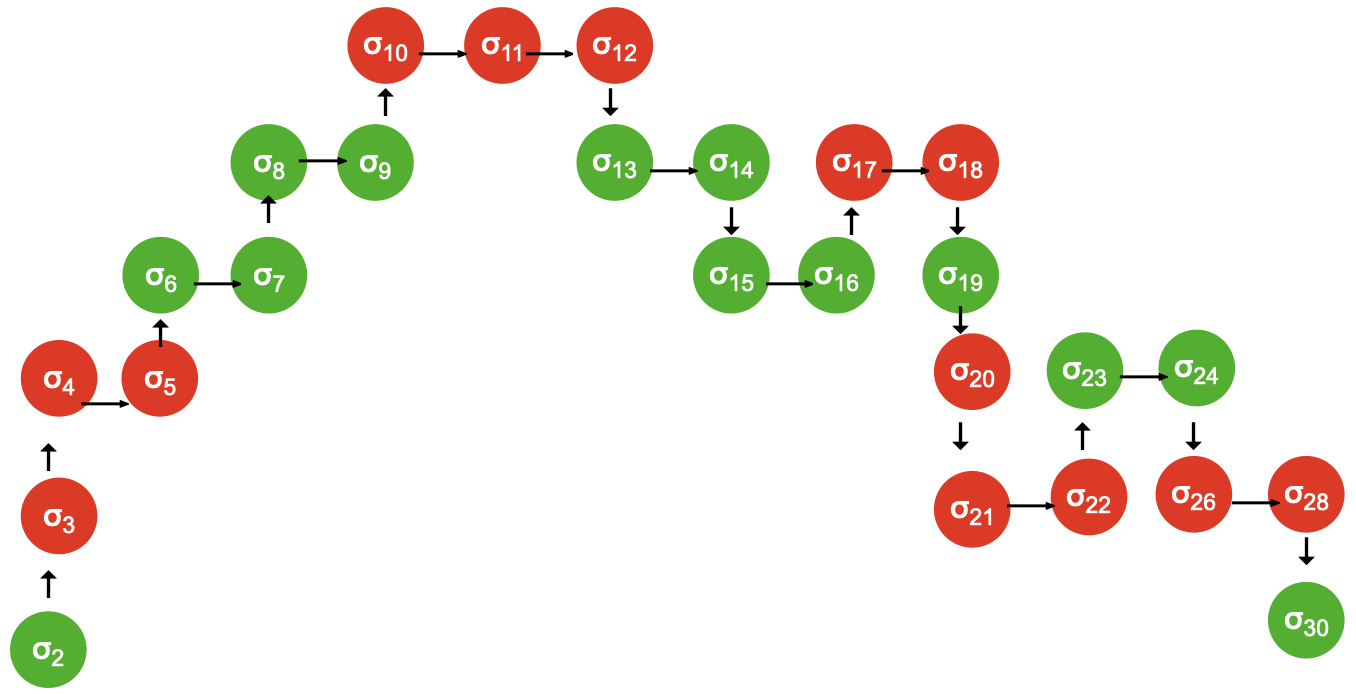
\includegraphics[width=\linewidth]{diagrams/summaryA.png}
} 
& &
\resizebox{6.2cm}{!}
{
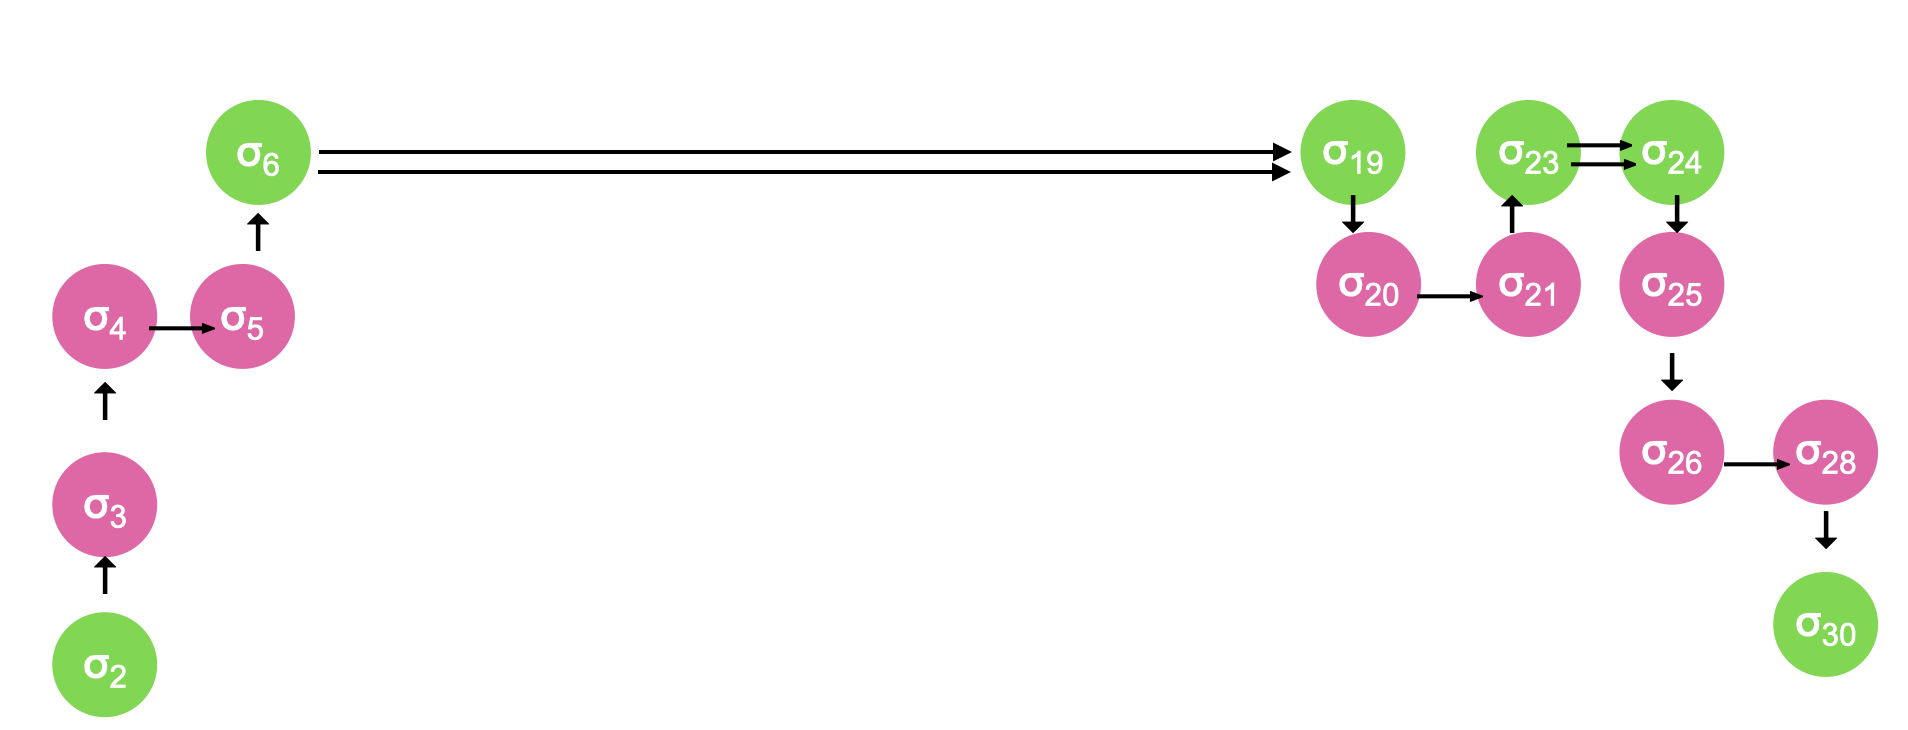
\includegraphics[width=\linewidth]{diagrams/summaryB.png}
} 
\end{tabular}
   \caption{Summaries. 
   }
   \label{fig:summariesNew}
 \end{figure}

The lemma  \ref{lemma:external_exec_preserves_more} describes how an encapsulated assertion $A$ is preserved during an execution, provided that all finalizing internal executions preserved it. 
It will be used in the proof of soundness of the rule {\sc{ExtCall\_WithSpec\_Weak}}\footnoteSD{perhaps also {\sc{ExtCall\_WithSpec\_Strong}}}



\begin{auxLemma}
\label{lemma:external_exec_preserves_more}[Preservation of Encapsulated Assertions]
For any module $M$, modules $\Mtwo$, variables $\overline x$, and addresses $\overline \alpha$,
 states $\sigma\bd$, $\sigma$, and $\sigma'$, and assertions $A$, $A'$, 
assume that

\noindent
 $M \models \encaps A \   \wedge  \ A'\txteq A[\overline{\alpha/x}]\  \wedge \ fv(A')=\emptyset \  \wedge \ 
M, \sigma \models  A' $. Then

\begin{enumerate}

\item
$   \leadstoBoundedThreeStarExt {\Mtwo\cdot M} {\sigma\bd}  {\sigma}  {\sigma'} 
\ \ \Longrightarrow \ \ \ M, \sigma' \models A'$

\item
$M, \sigma  \models \extThis \ \wedge \  \leadstoBoundedThree  {\Mtwo\cdot M} {\sigma} {\sigma}  {\sigma_{1}} \ \wedge
 \ M, \sigma_1 \models \pubMeth \ \wedge\  \leadstoBoundedStarFin {\Mtwo\cdot M} {\sigma_1}  {\sigma_2}    \ \ \wedge$\\
$ M, \sigma_2 \models A' \ \wedge \ 
  \   \leadstoBounded  {\Mtwo\cdot M} {\sigma_2}      {\sigma'}$\\
 $\Longrightarrow $
\\
$M, \sigma' \models A' $

\item
$ \WithExtPub {\Mtwo\cdot M} {\sigma\bd}  {\sigma}  {\sigma'} {\sigma_1...\sigma_n}\ \ \wedge $\\
 $\strut \ \ \ \  \  \forall i\in [1..n]. \forall \sigma_{f}.[ \ \  M, \sigma_i \models A'  \ \wedge \  \leadstoBoundedStarFin {M\cdot \Mtwo}  {\sigma_i}  {\sigma_{f}} \ 
\Longrightarrow \  M, \sigma_f \models A' \ ]$\\
$\Longrightarrow $
\\
$M, \sigma' \models A' $
\end{enumerate}

TOTHINK: Do we also need that $A$ is a module invariant?
\end{auxLemma}






%%%

  %%%%%%%%%%%%%%%%%%%%%%%%%%%%%%%%%%%%%%%%%%%%%%%%%%%

\subsection{ Soundness of Hoare Quadruples Logic, and the overall system}
\label{sect:prove:sound:quadruples}
We now prove soundness of the inference system $M \vdash  \quadruple A {stmt} {A'} {A''}$:


\begin{theorem}
\label{t:quadruple:sound}
For module  $M$ % and $\Mtwo$, 
such that  $\vdash M$, and for any assertions $A$ and $A'$, and state  $\sigma$, we have

\begin{center}
$M\ \vdash\  \quadruple {A} {stmt} {A'} {A''}$ \ \ \ \ implies \ \ \ \ $M\ \modelsD\  \quadruple {A} {stmt} {A'} {A''}$
\end{center}

\end{theorem}

  %%%%%%%%%%%%%%%%%%%%%%%%%%%%%%%%%%%%%%%%%%%%%%%%%%%
%  \subsection{Soundness of the overall system}
\label{sect:prove:triples:overall}
Finally, we can now prove soundness of the overall system

\begin{theorem}[Soundness]
\label{thm:soundness}
%Assume an \SpecO proof system, $\proves{M}{A}$, 
%an encapsulation inference system, $\proves{M}{\encaps{A}}$,
%% Axiom xx, and 
% and  that on top of these systems we built
% the \SpecLang logic according to zzzz,  then, for    all modules $M$, and all \SpecLang specifications  $S$:
 For any module $M$, and specification $S$:
 
 $$\proves{M}{S}\ \ \ \ \ \ \ \mbox{implies}\ \ \ \ \ \  \ \ \ \satisfies{M}{S}$$
\end{theorem}

Proof sketches for these theorems can be found in \A, \ref{s:app:proof:sketch;quadruples}, and \ref{s:app:proof:sketch;overall}. 

%
%Theorem. \ref{thm:soundness} demonstrates 
% that the   \SpecLang logic is sound with respect to the semantics of \SpecLang specifications.
% The \SpecLang logic parametric wrt to the algorithms for proving validity of assertions
% $\proves{M}{A}$, and 
% assertion encapsulation ($\proves{M}{\encaps{A}}$), and is sound
% provided that these two proof systems are sound.
